\documentclass{report}
\author{Alasdair Macindoe}
\date{}
\title{Work Package 5.2: A Report}
\usepackage{hyperref}
\usepackage{listings}
\usepackage{pgfplots}
\lstset{
  numbers = left,
  tabsize = 1,
  stepnumber = 1,
  breaklines=true,
}

\begin{document}
\maketitle

\section*{Acknowledgements}
We acknowledge financial support from the \href{http://opendreamkit.org/}{OpenDreamKit} \href{https://ec.europa.eu/programmes/horizon2020/}{Horizon 2020}
\href{https://ec.europa.eu/programmes/horizon2020/en/h2020-section/european-research-infrastructures-including-e-infrastructures}{European Research Infrastructures}
project (\href{http://cordis.europa.eu/project/rcn/198334_en.html}{\#676541}).
Further we would like to thank \href{https://www.cs.st-andrews.ac.uk/directory/person?id=mp397}{Dr Markus Pfeiffer} for his supervision and all his help that was invaluable for this project.

\section*{Introduction}
Whilst enumerating finite semigroups is computationally expensive there are algorithms that can run - in a practical sense - faster than naively enumerating the semigroup. One example of this algorithm was published in 1997 by Froidure and Pin\cite{fpin} (which will henceforth be called the Froidure-Pin algorithm).
Unfortunately this algorithm does not leverage modern CPU architecture that are multi-cored; this is a huge problem for modern computational problems, hence this lead to another version of Froidure-Pin to be published\cite{cfp} (which we will henceforth call the parallel Froidure-Pin) which can run in parallel and for which a C++ implementation exists\cite{cfpcpp}.

\subsection*{Aim}
The aim of this project was to re-implement the parallel Froidure-Pin algorithm in HPC-GAP\cite{GAP4} and analyse its scalability.
The full repository for this project can be found on Github\cite{project}. This code was then shared to the general public under
the GNU GPL v3 license.

\section*{Structure}
All the code can be located on Github\cite{project}. The following auxiliary documentation may be of interest:
\newline
\begin{description}
\item \texttt{README.md}: Installation and testing instructions
\item \texttt{versions.md}: Explanation of implementation details
\item \texttt{runtimes.md}: Raw data from experiments
\item \texttt{data.md}: Explanation of different semigroups for testing
\item \texttt{experiment.g}: File to run experiments
\item \texttt{gap/}: Various implementations
\item \texttt{tst/}: The test file
\end{description}

Although summaries are given here. 

\section*{Failed Attempts and Approach}
This was a very challenging project, and there are many attempts before we arrived at \texttt{Version 2.1} which were failures.
The first attempt was creating in GAP the simplistic \texttt{naiveenumeration} variation, then from there work on implementing the
Froidure-Pin algorithm itself.
\newline
The real difficulty began with the parallel Froidure-Pin algorthim which was written in some very dense mathematical notation.
We have an attempt named \texttt{concurrentfp} where we completely misunderstood the algorithm, this lead us to have \texttt{Version 1.x} which whilst
does perform the job correctly it is not truly parallel at every stage and requires locking.
The insights gained from these failures did allow us to produce \texttt{Version 2.1} which we are incredibly happy with.
\newline
Overall we feel like this approach was the most beneficial. Not only did it require learning about semigroups and GAP, but it allowed us
to start from the beginning and develop our way through the approaches done throughout the years and improve and learn ourselves from our failures.

\section*{Implementation}
\texttt{Version 2.1} is an exact implementation of the version given in the paper. Here we will explain the decision we have made. 
It is very important to note that the three main functions all run sequentially. It is the functions themselves that are parallelised. 

\subsection*{Bucket Function}
The parallel Froidure-Pin algorthim makes an important decision: The bucket (that is the list of words that might be new) that a specific word is placed in deterministic. This means that there is no need to search through every bucket to see if a word exists at a later stage because it can only exist in one queue thus avoiding locking. 
\newline
Unfortunately HPC-GAP does not have a hash function for transformations hence an approximate implementation was done by us and it is most likely imperfect.

\subsection*{Fragment}
The paper has a very detailed explanation of what a fragment is but from a computational perspective a fragment is very simplistic. It is simply a collection of (unique - both within and outside the fragment) words and a K value (which will store the first unused word in the fragment). 
\newline
We choose to store Fragments in lists because HPC-GAP does not contain a good hashtable datastructure for transformations. There is an added benefit that whenever fragments are used they are either only read (inside ApplyGenerators), each fragment is used by at most one process (inside ProcessQueues), or each fragment is only read to find a word which is only in one process (inside DevelopLeft).

\subsection*{Word}
The word datastructure contains a lot of attributes. This is done because it means that we often perform lookups instead of computations and since the parallel Froidure-Pin naturally used a lot of memory a small amount extra to reduce runtime seemed like a good trade off. It also makes nicer computational sense. 

\subsection*{Apply Generators}
This explanation is a direct copy from \texttt{Versions.md}. 
\newline
Each instance of Apply Generators created (one per task) deals with a specific fragment of reduced words (`Y` is the set of all fragments and internally `Yj` is used for the jth fragment). It uses the K value defined within that fragment to iterate until we have exceeded the size of the fragment (note that at this stage we are never increasing the size of fragments) or the word we are currently on is above the length that we are currently iterating over. We do not require a lock on the fragment `Yj` because it is only being used in one thread; the thread with the `jth` job assigned to it.

We then require the Kth word for that fragment (internally called `YjKj`) which you may notice we do not need to lock either because for each job (which gets its own task) the iteration is sequential across the words which means each thread is accessing at most one word in its fragment's words at any time. For every generator we perform a series of instructions. Firstly we check to see if its suffix's right multiple by this generator is reduced or not and if it is not reduced then we reduce it.

Secondly we find the right multiple of this word with that generator and see if it exists within the fragment we are assigned to. Note that no locking is required at this point since we are not ever editing anything within the set of reduced words and if we do amend a word it is specific to that task which means no other job will be trying to access it.
If the word exists then its right multiple is updated, otherwise we create a new word with that value (which gives it a bucket number) and add it to that bucket and added to that jobs queue for Process Queues.
Further note that a word may exist in another fragment but this will be dealt with by Process Queues and this means that not all values placed into the queue will actually be unique - this is done to avoid any locking.

\subsection*{Process Queues}
This explanation is a direct copy from \texttt{Versions.md}. 
\newline
In order to remove the requirement for locking the implementation makes each `ProcessQueues` loop over every word in every queue (this is read only because we do not update the words inside `ProcessQueues`) and then perform the merging steps on words that have the bucket entry corresponding to its job number (this means each `ProcessQueues` instances deals with a different bucket meaning no concurrency issues arise). This works because each word (until the inner part) is read only and since each word can only have one bucket (and each instance has a different bucket) there can be no race conditions when we merge the word (no other task has this word and no other task is using this bucket). Additionally notice that the bucketing function is deterministic this means that any identical words are put in the same bucket even if they have different queue numbers meaning that two tasks will never attempt to add the same word.
For clarity: We are adding any unique word (from all fragments) to a specific fragment which is what ever task has the bucket that word is assigned to.

\subsection*{Process Queues}
This explanation is a direct copy from \texttt{Versions.md}. 
\newline
The paper does not define `DevelopLeft` but we believed the code looked neater if it was abstracted to its own function. `DevelopLeft` develops the left Caley graph for each newly added word as well as performing any reductions of older words. Each task of `DevelopLeft` deals with exactly one of the fragments (which at this stage all have unique words). Occasionally words in other fragments may need to accessed but it is read only in this task and the part of the word we care about (the prefix) is never updated once set allowing us to do this safely.
\section*{Analysis}
Please refer to \texttt{runtimes.md} for the raw data, only summaries are provided below.
\newline
All experiments are on implementation \texttt{Version 2.x}.
\newline
The semigroup used can be found in the appendix as can the machine specifications. 

\subsection*{Experiment 1}
The aim of this experiment was to see the effect of increasing the number of core available without increasing the number of fragments.
\newline
We believe this was worth investigating because HPC-GAP's Task implementation is not guaranteed 1 to 1 with processes.
\newline
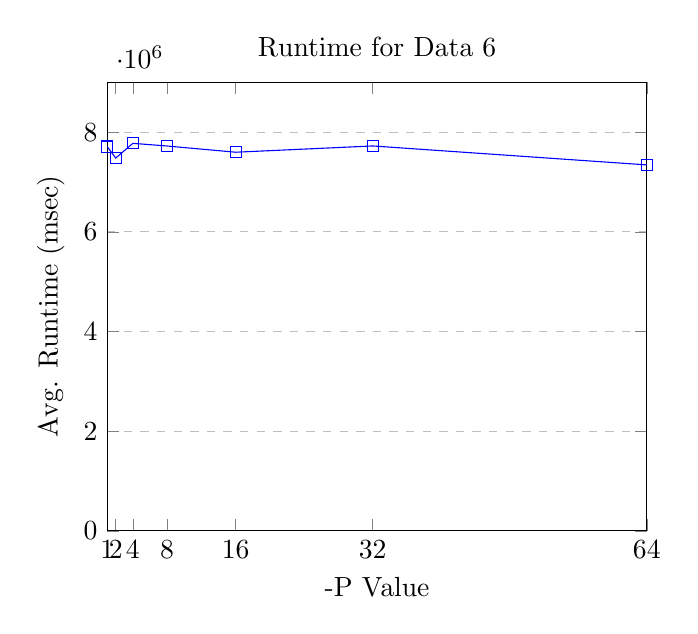
\begin{tikzpicture}
\begin{axis}[
    title={Runtime for Data 6},
    xlabel={-P Value},
    ylabel={Avg. Runtime (msec)},
    xmin=1, xmax=64,
    ymin=0, ymax=9000000,
    xtick={1, 2, 4, 8, 16, 32, 64},
    ymajorgrids=true,
    grid style=dashed,
]
 
\addplot[
    color=blue,
    mark=square,
    ]
    coordinates {
    (1, 7713242)(2, 7483817)(4, 7778529)(8, 7724759)(16, 7600084)(32, 7725967)(64, 7345427)
    };
 
\end{axis}
\end{tikzpicture}

From this we can see that there is no effect on the runtime when we just vary the number of core available without changing the number of fragments.

\subsection*{Experiment 2}
The aim of this experiment was to instead see how the number of fragments effects the runtime. We keep P = 32 for all attempts.
\newline
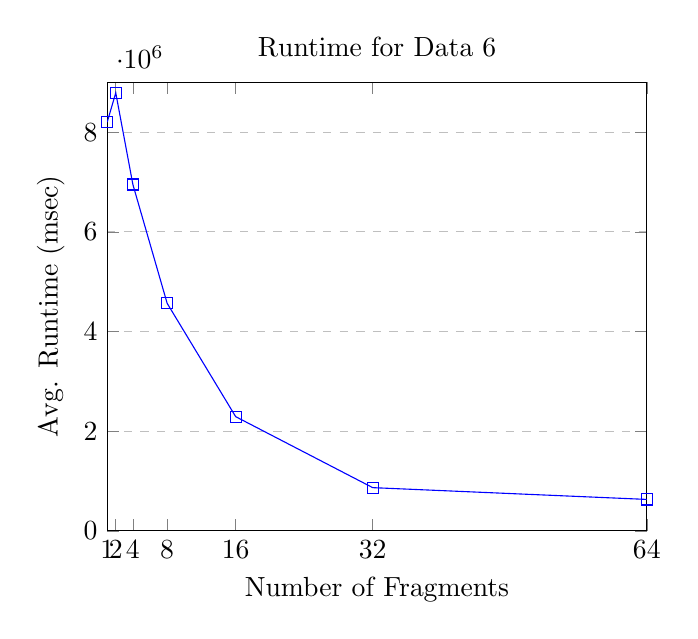
\begin{tikzpicture}
\begin{axis}[
    title={Runtime for Data 6},
    xlabel={Number of Fragments},
    ylabel={Avg. Runtime (msec)},
    xmin=1, xmax=64,
    ymin=0, ymax=9000000,
    xtick={1, 2, 4, 8, 16, 32, 64},
    ymajorgrids=true,
    grid style=dashed,
]
 
\addplot[
    color=blue,
    mark=square,
    ]
    coordinates {
    (1, 8202761)(2, 8792324)(4, 6952345)(8, 4567620)(16, 2291670)(32, 866321)(64, 629930)
    };
 
\end{axis}
\end{tikzpicture}
\newline
This very clearly has an impact even beyond the number of cores available. 

\begin{table}[]
\centering
\begin{tabular}{ccc}
\multicolumn{1}{l}{\textbf{Cores}} & \multicolumn{1}{l}{\textbf{Percentage of half cores}} & \textbf{Percentage of base} \\
1                                  & -                                                     & 100                         \\
2                                  & 107                                                   & 107                         \\
4                                  & 79                                                    & 85                          \\
8                                  & 65                                                    & 55                          \\
16                                 & 50                                                    & 28                          \\
32                                 & 37                                                    & 11                          \\
64                                 & 72                                                    & 8                          
\end{tabular}
\end{table}
This clearly shows that the rate of decrease in time becomes faster as we approach the number of cores and fragments being equal, it further shows that this rate decreases once we exceed that. Further experimentation may show that this trend reverses as we dramatically exceed our -P value. 
\newline
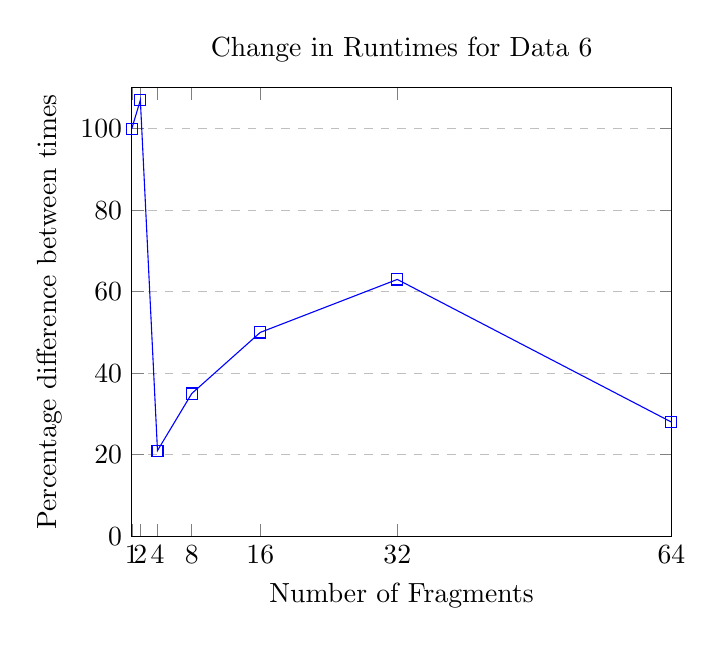
\begin{tikzpicture}
\begin{axis}[
    title={Change in Runtimes for Data 6},
    xlabel={Number of Fragments},
    ylabel={Percentage difference between times},
    xmin=1, xmax=64,
    ymin=0, ymax=110,
    xtick={1, 2, 4, 8, 16, 32, 64},
    ymajorgrids=true,
    grid style=dashed,
]
 
\addplot[
    color=blue,
    mark=square,
    ]
    coordinates {
    (1, 100)(2, 107)(4, 21)(8, 35)(16, 50)(32, 63)(64, 28)
    };
 
\end{axis}
\end{tikzpicture}
\newline
The important part of this graph is that speed up for doubling the number of fragments is not linear, in fact it seems to have diminishing returns after a certain point. 
\subsection*{Explanation of Metrics}
Given the example of 4 fragment compared to 8 fragment then the metric 'Percentage of half cores' means what percentage of the runtime of 4 cores is the runtime of 8 cores.
\newline
For example $695234 \cdot 0.65 \approx ~4567620$ which gives us the scaling from doubling the number of fragments. 
\newline
Then the metric 'percentage of base' gives us what percentage of the runtime of 1 fragment is 8 fragments?
\newline
For example $8202761 \cdot 0.55 \approx ~4567620$
\newline
Any inaccuracies arise from rounding. 
\section*{Contributions to HPC-GAP}
A bug in HPC-GAP was discovered which would cause a segmentation fault when an empty list was attempted to be migrated between tasks.
This was fixed by Dr Markus Pfeiffer\cite{hpcsol}.

\section*{Future Work}
We have identified some potential future works that could be done:

\begin{enumerate}
\item Fix any outstanding bugs and perform more significant testing especially relating to undiscovered bugs in HPC-GAP
\item Covert data structures across to the HPC-GAP's datastructures package\cite{ds}
\item Investigate performance increases by using HPC-GAP's threads and processes API
\item Investigate performance increases in HPC-GAP's tasks system
\item Investigate potential hash functions
\end{enumerate}

\section*{Conclusion}
In sum we have successfully implemented the parallel Froidure-Pin algorithm several times in HPC-GAP and compared their scalability.
Additionally we have identified bugs that exist within HPC-GAP and identified future work that could be conducted in this area.
\newline
We further believe that the skills honed here will allow us to make stronger Computer Scientists and software engineers.
\newline
The experimentation clearly shows that the algorithm's runtime scales reasonably well with large number of cores with the most dramatic speed ups occurring as we near the number of available cores. 

\section*{Appendix}

\section*{Research Server}
The research server 'Lovelace' has four CPUs with 16 cores each (giving 64 cores total), 32 16GB PC3-12800 DDR3-1600MHz ECC Ram (512 GB total). 

\section*{Data Source 6}
The semigroup used for experimentation was as follows:
\begin{lstlisting}
g := [ Transformation( [ 6, 7, 11, 8, 3, 8, 4, 6, 6, 9, 14, 10, 2, 5 ] ), Transformation( [ 9, 6, 12, 10, 12, 3, 5, 1, 5, 1, 12, 5, 5, 13 ] ) ];;
\end{lstlisting}
This semigroup has 124386 elements when fully enumerated. 
\bibliographystyle{plain}
\bibliography{citations}
\end{document}
